\documentclass[margin=0.2cm]{standalone}
\usepackage{graphicx}
\usepackage{amsthm}
\usepackage{amssymb,amsmath,amsbsy}
\usepackage{tikz-cd}
\usepackage{tikz}
\usetikzlibrary{automata,positioning}
%\usepackage{hyperref}
\usepackage{accents}
\usepackage{changepage}
\usepackage{stmaryrd}
\usepackage{thmtools}
\usepackage{xcolor}
\usepackage{pagecolor}


\pagecolor{black}
\color{white}

\begin{document}

%\begin{tikzcd}
%M_0 \arrow[rd, "f_0"] \arrow[rr, "id"] & & M_0 \\
%& W \arrow[ru, "i_0"] &
%\end{tikzcd}

%\begin{tikzpicture}[shorten >=1pt,node distance=2.9cm,initial text=,accepting/.style=accepting by double,auto] 
%  % Reachable states of the synchronous product of the 3 automata
%  \node[state,initial] (a00) {$ Q_0$};
%  \node[state] (a11) [below right=of a00] {$ Q_1$};
%  \node[state] (sink) [above left=of a00] {sink};
%  \node[state] (a01) [below left=of a00] {$ Q_2$};
%  \node[state,accepting] (as1) [above right=of a00] {$ Q_3$};
%
%  \path[->]
%    (a00) edge [loop right] node {X:0 Y:0,1} ()
%         edge node {X:1 Y:1} (a11)
%         edge node [swap] {X:1 Y:0} (sink)
%
%    (a01) edge [loop below] node {X:0 Y:0,1} ()
%          edge node {X:1 Y:0} (sink)
%
%    (a11) edge node {X:0 Y:1} (a01)
%         edge node [swap] {X:0 Y:0} (as1)
%         edge [bend left] node {X:1 Y:0,1} (sink)
%
%    (as1) edge [loop above] node {X:0 Y:0,1} ()
%          edge node [swap] {X:1 Y:0} (sink)
%    ;
%\end{tikzpicture}

%\begin{tikzpicture}[initial where=above,shorten >=1pt,node distance=2.9cm,initial text=,accepting/.style=accepting by double,auto]
%  % Determinized DFA via subset construction
%  \node[state,initial] (D0)  {$\{Q_0\}$};
%  \node[state] (D1) [left=of D0] {$\{Q_0,\;Q_4\}$};
%  \node[state] (D2) [right=of D0] {$\{Q_0,\;Q_1\}$};
%
%  \node[state] (D3) [below=of D1] {$\{Q_0,\;Q_1,\;Q_4\}$};
%  \node[state] (D4) [below=of D0,accepting] {$\{Q_0,\;Q_4,\;Q_3\}$};
%  \node[state] (D5) [below=of D2] {$\{Q_0,\;Q_1,\;Q_2,Q_4\}$};
%
%  \node[state,accepting] (D6) [below=of D4] {$\{Q_0,\;Q_1,\;Q_3,\;Q_4\}$};
%  \node[state,accepting] (D7) [below right=of D6] {$\{Q_0,\;Q_2,\;Q_3,\;Q_4\}$};
%  \node[state,accepting] (D8) [below left=of D6] {$\{Q_0,\;Q_1,\;Q_2,\;Q_3,\;Q_4\}$};
%
%  \path[->]
%    % D0 = {q0}
%    (D0) edge node {Y:0} (D1)
%         edge node {Y:1} (D2)
%
%    % D1 = {q0,sink}
%    (D1) edge [loop above] node {Y:0} ()
%         edge node {Y:1} (D3)
%
%    % D2 = {q0,q1}
%    (D2) edge node {Y:0} (D4)
%         edge node {Y:1} (D5)
%
%    % D3 = {q0,q1,sink}
%    (D3) edge node {Y:0} (D4)
%         edge [bend right] node {Y:1} (D5)
%
%    % D4 = {q0,sink,q3} (accepting)
%    (D4) edge [loop above] node {Y:0} ()
%         edge [bend right] node {Y:1} (D6)
%
%    % D5 = {q0,q1,q2,sink}
%    (D5) edge node {Y:0} (D7)
%         edge [loop right] node {Y:1} ()
%
%    % D6 = {q0,q1,q3,sink} (accepting)
%    (D6) edge [bend right] node {Y:0} (D4)
%         edge [bend right] node {Y:1} (D8)
%
%    % D7 = {q0,q2,q3,sink} (accepting)
%    (D7) edge [loop below] node {Y:0} ()
%         edge [bend left] node {Y:1} (D8)
%
%    % D8 = {q0,q1,q2,q3,sink} (accepting)
%    (D8) edge [bend left] node {Y:0} (D7)
%         edge [loop below] node {Y:1} ()
%    ;
%\end{tikzpicture}

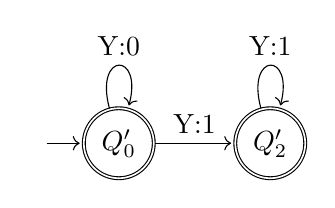
\begin{tikzpicture}[shorten >=1pt,node distance=1cm,initial text=,accepting/.style=accepting by double,auto]
  % Determinized DFA via subset construction
  \node[state,initial, accepting] (D0)  {$Q'_0$};
  \node[state, accepting] (D5) [right=of D0] {$Q'_2$};

  \path[->]
    % D0 = {q0}
    (D0) edge [loop above] node {Y:0} ()
         edge node {Y:1} (D5)

    % D5 = {q0,q1,q2,sink}
    (D5) edge [loop above] node {Y:1} ()
     ;
\end{tikzpicture}


\end{document}